\chapter{IPFS}

IPFS stands for InterPlanetary File System and is a peer-to-peer distributed filesystem designed to make the Web faster, safer, and more open. In contrast with standard filesystems, objects in IPFS are content-addressed, by the cryptographic hash of their contents. In the case of the standard Web, when user wants some file, he needs to know on which server is a file located and the full path to the file (see figure \ref{webAddressing}). In IPFS user needs only to know the hash of the requested file. He does not care about the location of the file (see figure \ref{ipfsAddressing}). Let’s take a very famous file, and add it to IPFS. Here’s the plain-text MIT license:

\begin{figure}[H]
    \texttt{Permission is hereby granted, free of charge, to any person obtaining a copy of this software and associated documentation files (the "Software"), to deal in the Software without restriction, including without limitation the rights to use, copy, modify, merge, publish, distribute, sublicense, and/or sell copies of the Software, and to permit persons to whom the Software is furnished to do so, subject to the following conditions:\\\\ The above copyright notice and this permission notice shall be included in all copies or substantial portions of the Software.\\\\ THE SOFTWARE IS PROVIDED "AS IS", WITHOUT WARRANTY OF ANY KIND, EXPRESS OR IMPLIED, INCLUDING BUT NOT LIMITED TO THE WARRANTIES OF MERCHANTABILITY, FITNESS FOR A PARTICULAR PURPOSE AND NONINFRINGEMENT. IN NO EVENT SHALL THE AUTHORS OR COPYRIGHT HOLDERS BE LIABLE FOR ANY CLAIM DAMAGES OR OTHER LIABILITY, WHETHER IN AN ACTION OF CONTRACT, TORT OR OTHERWISE, ARISING FROM, OUT OF OR IN CONNECTION WITH THE SOFTWARE OR THE USE OR OTHER DEALINGS IN THE SOFTWARE.}
\end{figure}

\noindent If somebody will try to add this license as file to IPFS, it will return \texttt{QmWpvK4bYR7k9b1feM48fsk\-t2XsZfMaPfNnFxdbhJHw7QJ} every time. That is now, and will be in the future, the \textit{content address} of that file. Later, when you try to get this file by it's hash, you can get it from random person that added it into IPFS the past.


\begin{figure}[h]
    \centering
    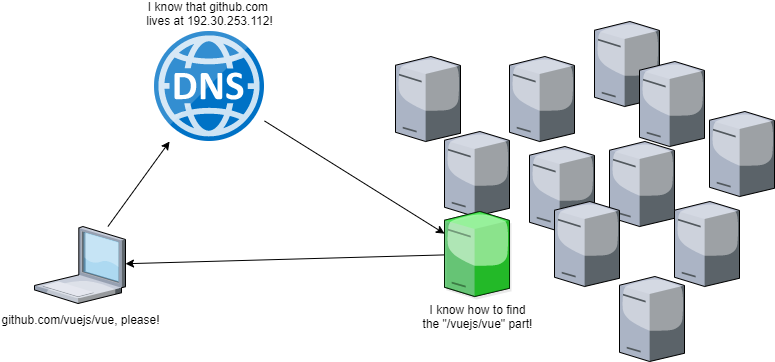
\includegraphics[width=11cm]{classicWebAddresing.png}
    \caption{Classic web addresing}
    \label{webAddressing}
\end{figure}

\begin{figure}[h]
    \centering
    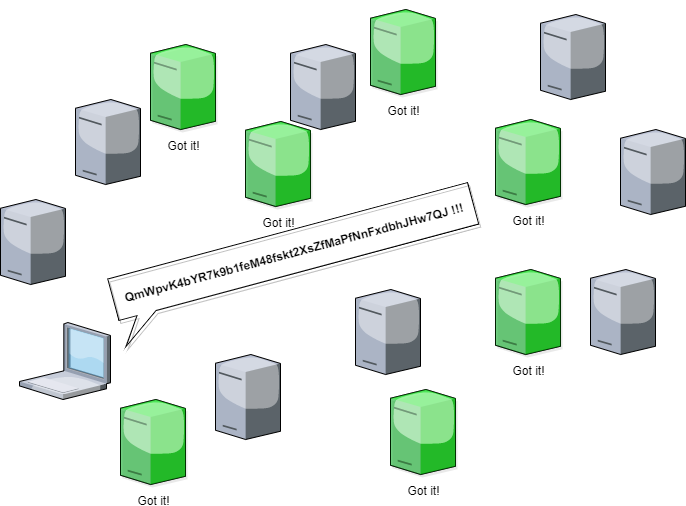
\includegraphics[width=11cm]{ipfsAddressing.png}
    \caption{Content-based addressing}
    \label{ipfsAddressing}
\end{figure}

\section{IPFS stack}
Like in other network models, we can IPFS split into layers (see figure \ref{IPFSstack}). There is \textit{libp2p}\footnote{\url{https://libp2p.io/}} at the bottom which is peer-to-peer networking module, that handle peer and content discovery, transport, security, identity, peer routing and messaging. \textit{IPLD} is the data model of the content-addressable web. It providing linking between objects and multihash computing. On the top is \textit{IPFS} which allows to publish and share files (or any data).\cite{IPFSwhitepaper}


\begin{figure}[h]
    \centering
    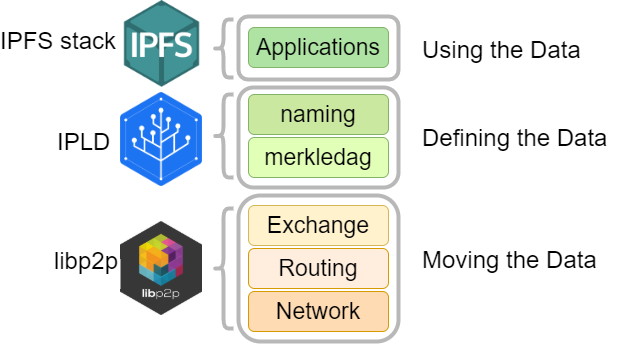
\includegraphics[width=11cm]{IPFSstack.png}
    \caption{IPFS stack}
    \label{IPFSstack}
\end{figure}


\subsection{libp2p}
\subsection{IPLD}
\subsection{IPFS}


